\lab{Kalman Filter}{Kalman Filter}
\objective{Understand how to implement the standard Kalman Filter. Apply to the problem of projectile tracking.}

Measured observations are often prone to significant noise, due to restrictions on measurement accuracy.
For example, most commercial GPS devices can provide a good estimate of geolocation, but only within a dozen meters or so.
A Kalman filter is an algorithm that takes a sequence of noisy observations made over time and attempts to get rid of the noise,
producing more accurate estimates than the original observations.
To do this, the algorithm needs information about the system being observed.

Consider the problem of tracking a projectile as it travels through the air.
Short-range projectiles approximately trace out parabolas, but a sensor that is recording measurements of the projectile's position over time will likely show a path that is much
less smooth.
Because we know something about the laws of physics, we can filter out the noise in the measurements using basic Newtonian mechanics, recovering a more accurate estimate
of the projectile's trajectory.
In this lab, we will simulate measurements of a projectile and implement a Kalman filter to estimate the complete trajectory of the projectile.

\section*{Linear Dynamical Systems}
The standard Kalman filter assumes that:
(1) we have a linear dynamical system,
(2) the state of the system evolves over time with some noise, and
(3) we receive noisy measurements about the state of the system at each iteration.
More formally, letting $\mathbf{x}_{k}$ denote the state of the system at time $k$, we have
\begin{equation}
\mathbf{x}_{k+1} = F_{k} \mathbf{x}_{k} + B_{k}\mathbf{u}_{k} + \boldsymbol{\epsilon}_{k}
\label{eq:state}
\end{equation}
where $F_{k}$ is a state-transition model, $B_{k}$ is a control-input model, $\mathbf{u}_{k}$ is a control vector, and $\boldsymbol{\epsilon}_{k}$ is the noise present in state $k$.
This noise is assumed to be drawn from a multivariate Gaussian distribution with zero mean and covariance matrix $Q_{k}$.
The control-input model and control vector allow the assumption that the state can be additionally influenced by some other factor than the linear state-transition model.

We further assume that the states are ``hidden,'' and we only get the noisy observations
\begin{equation}
\mathbf{z}_{k} = H_{k}\mathbf{x}_{k} + \boldsymbol{\delta}_{k}
\label{eq:obs}
\end{equation}
where $H_{k}$ is the observation model mapping the state space to the observation space, and $\boldsymbol{\delta}_{k}$ is the observation noise present at iteration $k$.
As with the aforementioned error, we assume that this noise is drawn from a multivariate Gaussian distribution with zero mean and covariance matrix $R_{k}$.

The dynamics stated above are all taken to be linear.
Thus, for our purposes, the operators $F_k$, $B_k$, and $H_k$ are all matrices, and $\mathbf{x}_k$, $\mathbf{u}_k$, $\mathbf{z}_k$, and $\boldsymbol{\delta}_k$ are all vectors.

We will assume that the transition and observation models, the control vector, and the noise covariances are constant, i.e. for each $k$, we will replace $F_{k}, H_k, \mathbf{u}_{k}, Q_{k},$ and $R_{k}$ with $F, H, \mathbf{u}, Q,$ and $R$.
We will also assume that $B = I$ is the identity matrix, so it can safely be ignored.

\begin{problem}
Begin implementing a \li{KalmanFilter} class by writing an initialization method that stores the transition and observation models, noise covariances, and control vector.
We provide an interface below:
\begin{lstlisting}
class KalmanFilter(object):
    def __init__(self,F,Q,H,R,u):
        """
        Initialize the dynamical system models.

        Parameters
        ----------
        F : ndarray of shape (n,n)
            The state transition model.
        Q : ndarray of shape (n,n)
            The covariance matrix for the state noise.
        H : ndarray of shape (m,n)
            The observation model.
        R : ndarray of shape (m,m)
            The covariance matric for observation noise.
        u : ndarray of shape (n,)
            The control vector.
        """
        pass
\end{lstlisting}
\end{problem}

We now derive the linear dynamical system parameters for a projectile traveling through $\mathbb{R}^2$ undergoing a constant downward gravitational force of 9.8 $m/s^2$.
The relevant information needed to describe how the projectile moves through space is its position and velocity.
Thus, our state vector has the form
\[
\mathbf{x} = \left( \begin{array}{c} s_{x} \\ s_{y} \\ V_{x} \\ V_{y} \end{array} \right),
\]
where $s_x$ and $s_y$ give the $x$ and $y$ coordinates of the position (in meters), and $V_x$ and $V_y$ give the horizontal and vertical components of the velocity (in meters per second), respectively.

How does the system evolve from one time step to the next?
Assuming each time step is $0.1$ seconds, it is easy enough to calculate the new position:
\begin{align*}
s_x' &= s_x + 0.1V_x\\
s_y' &= s_y + 0.1V_y.
\end{align*}
Further, since the only force acting on the projectile is gravity (we are ignoring things like wind resistance), the horizontal velocity remains constant:
\[
V_x' = V_x.
\]
The vertical velocity, however, does change due to the effects of gravity.
From basic Newtonian mechanics, we have
\[
V_y' = V_y - 0.1\cdot9.8.
\]
In summary, over one time step, the state evolves from $\mathbf{x}$ to $\mathbf{x}'$, where
\[
\mathbf{x}' = \left( \begin{array}{c} s_{x} + 0.1V_x \\ s_{y} + 0.1V_y \\ V_{x} \\ V_{y} - 0.98 \end{array} \right).
\]
From this equation, you can extract the state transition model $F$ and the control vector $u$.

We now turn our attention to the observation model.
Imagine that a radar sensor captures (noisy) measurements of the projectile's position as it travels through the air.
At each time step, the radar transmits the observation $z = (z_x, z_y)$ given by
\begin{align*}
z_x &= s_x + \delta_x\\
z_y &= s_y + \delta_y,
\end{align*}
where $(\delta_x, \delta_y)$ is a noise vector assumed to be drawn from a multivariate Gaussian with mean zero and some known covariance.
These equations indicate the appropriate choice of observation model.

\begin{problem}
Work out the transition and observation models $F$ and $H$, along with the control vector $\mathbf{u}$, corresponding to the projectile.
Assume that the noise covariances are given by
\begin{align*}
Q &= 0.1 \cdot I_4\\
R &= 5000 \cdot I_2.
\end{align*}
Instantiate a \li{KalmanFilter} object with these values.
\end{problem}

\begin{figure}
    \centering
    \begin{tabular}{cc}
    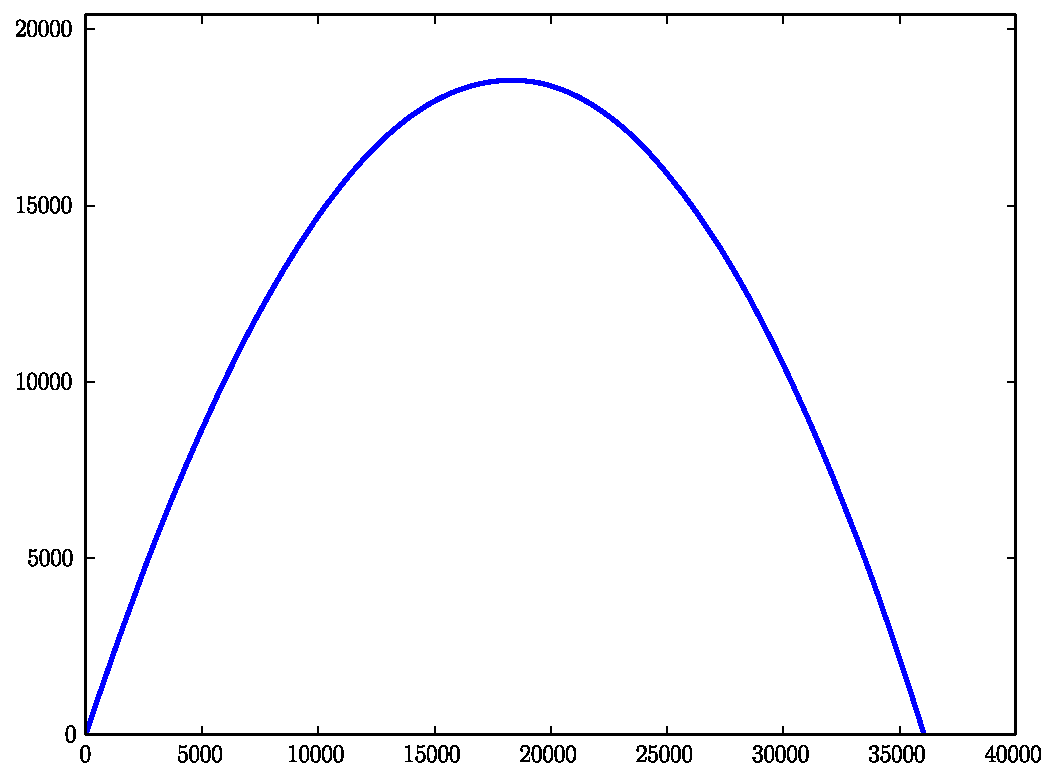
\includegraphics[width=.45\textwidth]{states_evolution} &
    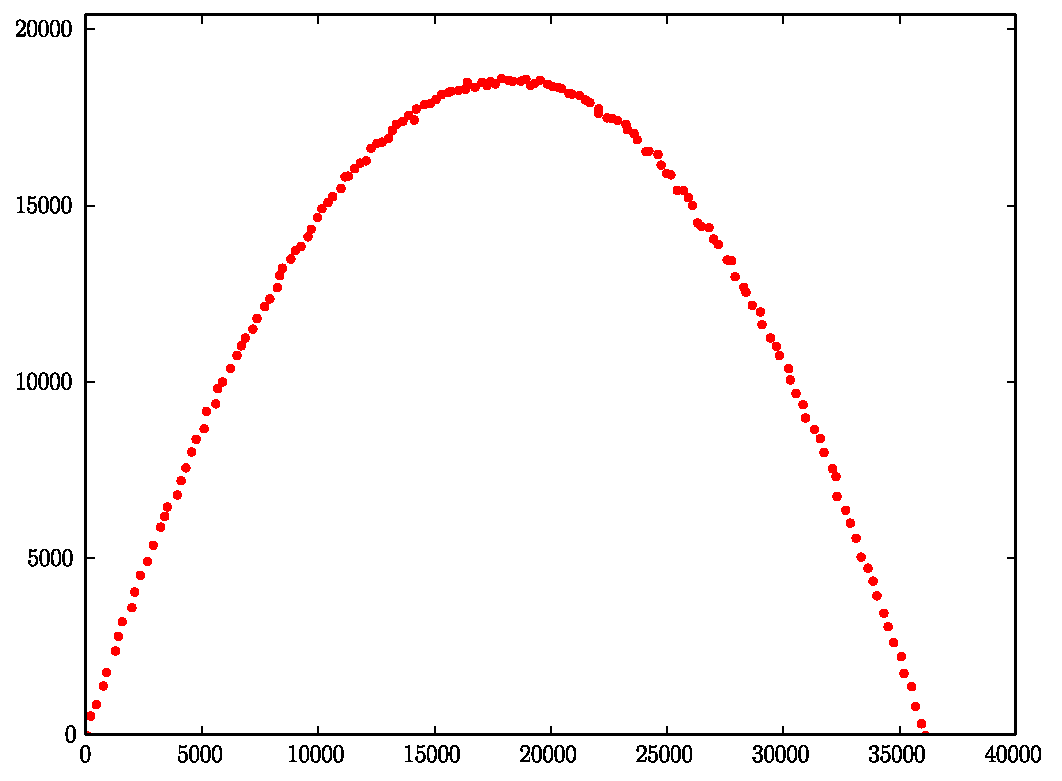
\includegraphics[width=.45\textwidth]{obs_evolution}
    \end{tabular}
    \caption{State sequence (left) and sampling of observation sequence (right).}
    \label{fig:evolution}
\end{figure}

We now wish to simulate a sequence of states and observations from the dynamical system.
In addition to the system parameters, we need an initial state $\mathbf{x}_0$ to get started.
Computing the subsequent states and observations is simply a matter of following equations \ref{eq:state} and \ref{eq:obs}.

\begin{problem}
Add a method to your \li{KalmanFilter} class to generate a state and observation sequence by evolving the system from a given initial state (the function \li{numpy.random.multivariate_normal} will be useful).
To do this, implement the following:
\begin{lstlisting}
def evolve(self,x0,N):
    """
    Compute the first N states and observations generated by the Kalman system.

    Parameters
    ----------
    x0 : ndarray of shape (n,)
        The initial state.
    N : integer
        The number of time steps to evolve.

    Returns
    -------
    states : ndarray of shape (n,N)
        States 0 through N-1, given by each column.
    obs : ndarray of shape (m,N)
        Observations 0 through N-1, given by each column.
    """
    pass
\end{lstlisting}

Simulate the true and observed trajectory of a projectile with initial state
\[
\mathbf{x}_0 = \left( \begin{array}{c} 0\\ 0 \\ 300 \\ 600\end{array} \right).
\]
Approximately 1250 time steps should be sufficient for the projectile to hit the ground (i.e. for the $y$ coordinate to return to 0).
Your results should qualitatively match those given in Figure \ref{fig:evolution}.
\label{prob:simulation}
\end{problem}



\section*{State Estimation with the Kalman Filter}
The Kalman filter is a recursive estimator that smooths out the noise in real time, estimating each current state based on the past state estimate and the current measurement.
This process is done by repeatedly invoking two steps: Predict and Update.
The predict step is used to estimate the current state based on the previous state.
The update step then combines this prediction with the current observation, yielding a more robust estimate of the current state.

To describe these steps in detail, we need additional notation. Let
\begin{itemize}
    \item $\widehat{\mathbf{x}}_{n|m}$ be the state estimate at time $n$ given only measurements up through time $m$; and
    \item $P_{n|m}$ be an error covariance matrix, measuring the estimated accuracy of the state at time $n$ given only measurements up through time $m$.
\end{itemize}

The elements $\widehat{\mathbf{x}}_{k|k}$ and $P_{k|k}$ represent the state of the filter at time $k$, giving the state estimate and the accuracy of the estimate.

%\begin{figure}
%    \centering
%    \includegraphics[width=.90\textwidth]{norms}
%    \caption{Norms of the estimated accuracy matrices as the Kalman filter progresses. }
%    \label{fig:norms}
%\end{figure}

We evolve the filter recursively, as follows:
\begin{align*}
\textbf{Predict} & & \widehat{\mathbf{x}}_{k|k-1} & = F\widehat{\mathbf{x}}_{k-1|k-1} + \mathbf{u} \\
 & & P_{k|k-1} & = FP_{k-1|k-1}F^{T} + Q \\
\textbf{Update} & & \tilde{\mathbf{y}}_{k} & = \mathbf{z}_{k} - H\widehat{\mathbf{x}}_{k|k-1} \\
 & & S_{k} & = HP_{k|k-1}H^{T} + R \\
 & & K_{k} & = P_{k|k-1}H^{T}S_{k}^{-1} \\
 & & \widehat{\mathbf{x}}_{k|k} & = \widehat{\mathbf{x}}_{k|k-1} + K_{k}\tilde{\mathbf{y}}_{k} \\
 & & P_{k|k} & = (I - K_{k}H)P_{k|k-1}
\end{align*}

The more observations we have, the greater the accuracy of these estimates becomes (i.e the norm of the accuracy matrix converges to $0$).
%This is reflected in Figure \ref{fig:norms}.

\begin{problem}
Add code to your \li{KalmanFilter} class to estimate a state sequence corresponding to a given observation sequence and initial state estimate.
Implement the following class method:
\begin{lstlisting}
def estimate(self,x,P,z):
    """
    Compute the state estimates using the Kalman filter.
    If x and P correspond to time step k, then z is a sequence of
    observations starting at time step k+1.

    Parameters
    ----------
    x : ndarray of shape (n,)
        The initial state estimate.
    P : ndarray of shape (n,n)
        The initial error covariance matrix.
    z : ndarray of shape(m,N)
        Sequence of N observations (each column is an observation).

    Returns
    -------
    out : ndarray of shape (n,N)
        Sequence of state estimates (each column is an estimate).
    """
    pass
\end{lstlisting}
\end{problem}

\begin{figure}
    \centering
    \begin{tabular}{cc}
    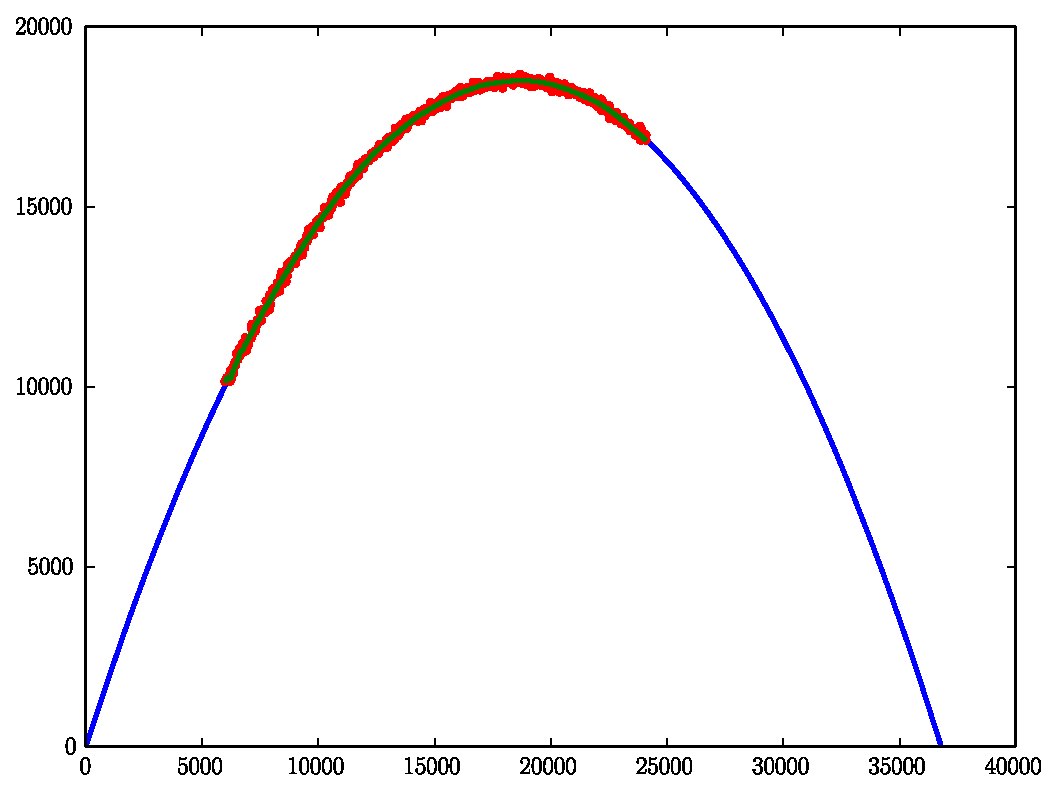
\includegraphics[width=.45\textwidth]{estimate_macro} &
    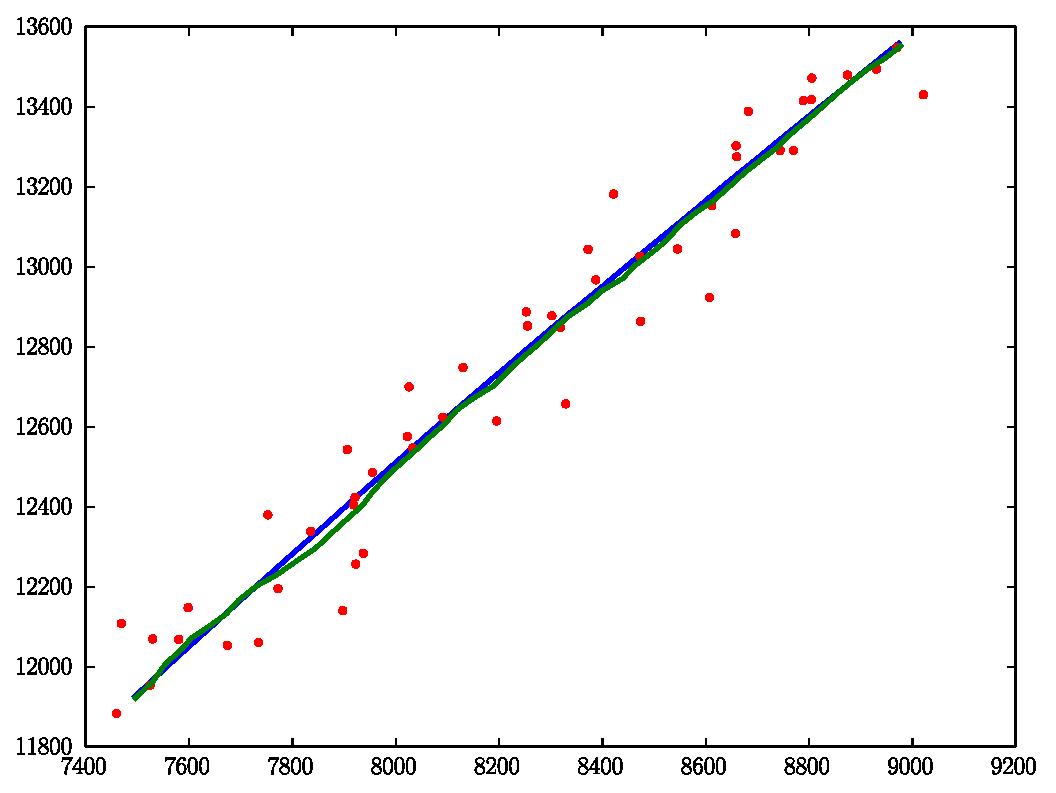
\includegraphics[width=.45\textwidth]{estimate_micro}
    \end{tabular}
    \caption{State estimates together with observations and true state sequence (detailed view on the right).}
    \label{fig:estimates}
\end{figure}

Returning to the projectile example, we now assume that our radar sensor has taken observations from time steps $200$ through $800$ (take the corresponding slice of the
observations produced in Problem \ref{prob:simulation}).
Using these observations, we seek to estimate the corresponding true states of the projectile.
We must first come up with a state estimate $\widehat{\mathbf{x}}_{200}$ for time step $200$, and then feed this into the Kalman filter
to obtain estimates $\widehat{\mathbf{x}}_{201}, \ldots, \widehat{\mathbf{x}}_{800}$.
\begin{problem}
Calculate an initial state estimate $\widehat{\mathbf{x}}_{200}$ as follows:
For the horizontal and vertical positions, simply use the observed position at time $200$.
For the velocity, compute the average velocity between the observations $\mathbf{z}_k$ and $\mathbf{z}_{k+1}$ for
$k = 200,\ldots,208$, then average these 9 values and take this as the initial velocity estimate.
(Hint: the NumPy function \li{diff} is useful here.)

Using the initial state estimate, $P_{200} = 10^{6} \cdot Q$, and your Kalman filter, compute the next $600$ state estimates,
i.e. compute $\widehat{\mathbf{x}}_{201}, \ldots, \widehat{\mathbf{x}}_{800}$.
Plot these state estimates as a smooth green curve together with the radar observations (as red dots) and the entire true state sequence (as a blue curve).
Zoom in to see how well it follows the true path. Your plots should be similar to Figure \ref{fig:estimates}.
\label{prob:state_estimate}
\end{problem}

In the absence of observations, we can still estimate some information about the state of the system at some future time.
We can do this by recognizing that the expected state noise $\mathbb{E}\left[\boldsymbol{\epsilon}_{k}\right] = 0$ at any time $k$.
Thus, given a current state estimate $\widehat{\mathbf{x}}_{n|m}$ using only measurements up through time $m$, the expected state at time $n+1$ is
\begin{equation*}
\widehat{\mathbf{x}}_{n+1|m} = F \widehat{\mathbf{x}}_{n|m} + \mathbf{u}
\end{equation*}

\begin{problem}
Add a function to your class that predicts the next $k$ states given a current state estimate but in the absence of observations.
Do so by implementing the following function:
\begin{lstlisting}
def predict(self,x,k):
    """
    Predict the next k states in the absence of observations.

    Parameters
    ----------
    x : ndarray of shape (n,)
        The current state estimate.
    k : integer
        The number of states to predict.

    Returns
    -------
    out : ndarray of shape (n,k)
        The next k predicted states.
    """
    pass
\end{lstlisting}
\end{problem}

\begin{figure}
    \centering
    \begin{tabular}{cc}
    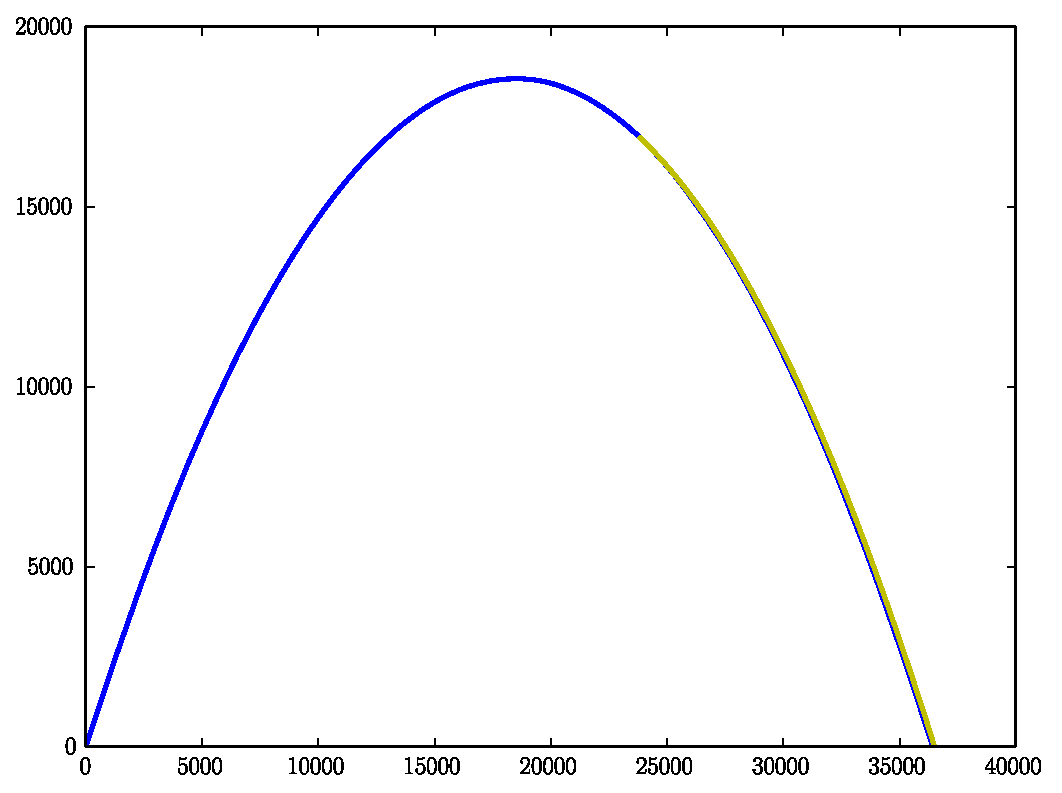
\includegraphics[width=.45\textwidth]{impact_macro} &
    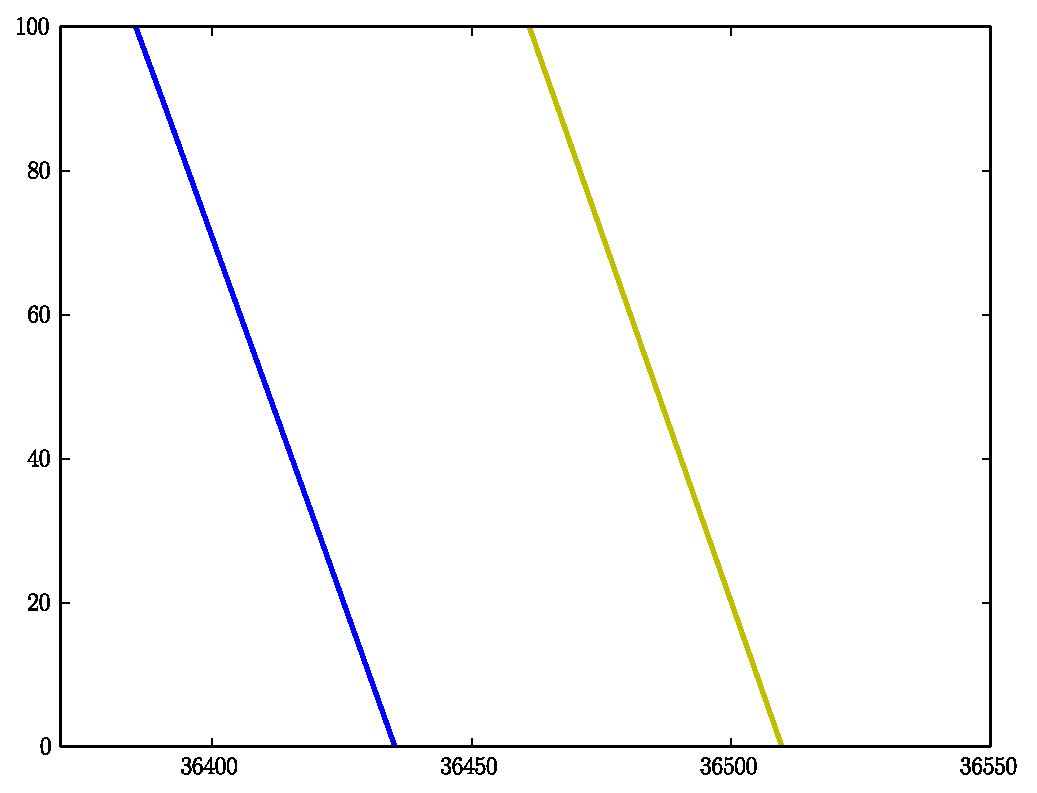
\includegraphics[width=.45\textwidth]{impact_micro}
    \end{tabular}
    \caption{Predicted vs. actual point of impact (detailed view on right).}
    \label{fig:impact}
\end{figure}

We can use this prediction routine to estimate where the projectile will hit the surface.
\begin{problem}
Using the final state estimate $\widehat{\mathbf{x}}_{800}$ that you obtained in Problem \ref{prob:state_estimate}, predict the future states of
the projectile until it hits the ground.
Predicting approximately the next $450$ states should be sufficient.

Plot the actual state sequence together with the predicted state sequence (as a yellow curve), and observe how near the prediction is to the actual point of impact.
Your results should be similar to those shown in Figure \ref{fig:impact}.
\end{problem}

In the absence of observations, we can also reverse the system and iterate backward in time to infer information about states of the system prior to measured observations.
The system is reversed by
\begin{equation*}
\mathbf{x}_{k} = F^{-1}(\mathbf{x}_{k+1} - \mathbf{u} - \boldsymbol{\epsilon}_{k+1}).
\end{equation*}
Considering again that $\mathbb{E}\left[\boldsymbol{\epsilon}_{k}\right] = 0$ at any time $k$, we can ignore this term, simplifying the recursive estimation backward in time.




\begin{figure}[htb]
    \centering
    \begin{tabular}{cc}
    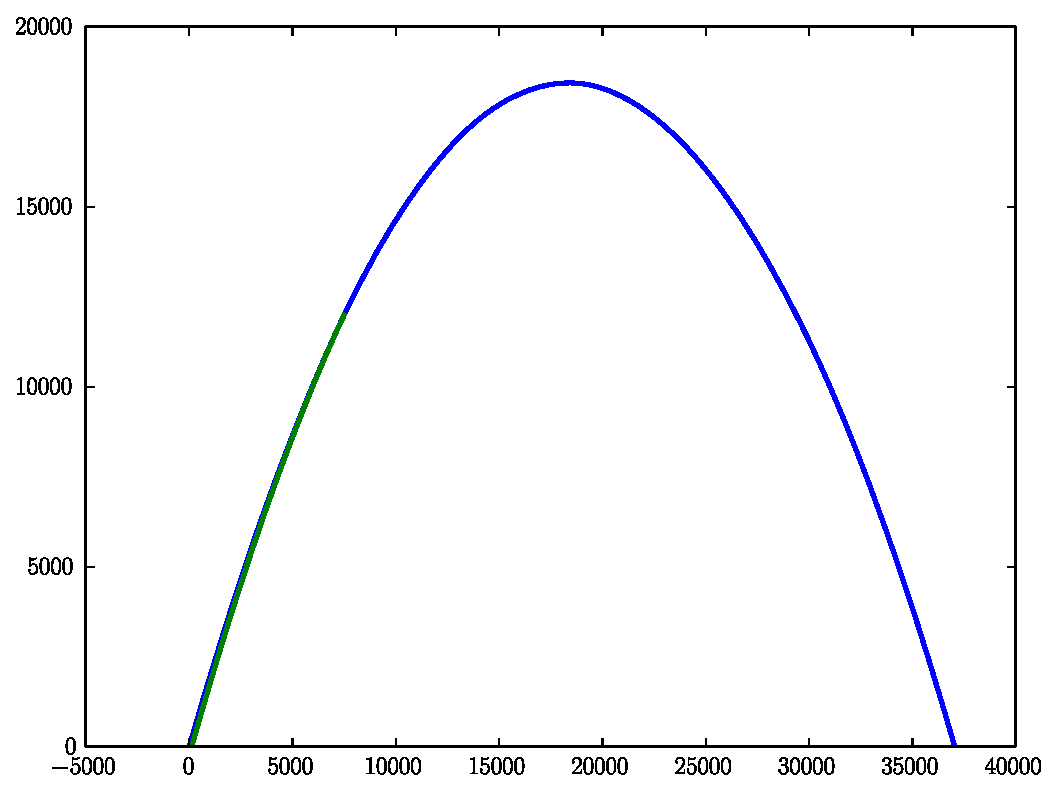
\includegraphics[width=.45\textwidth]{origin_macro} &
    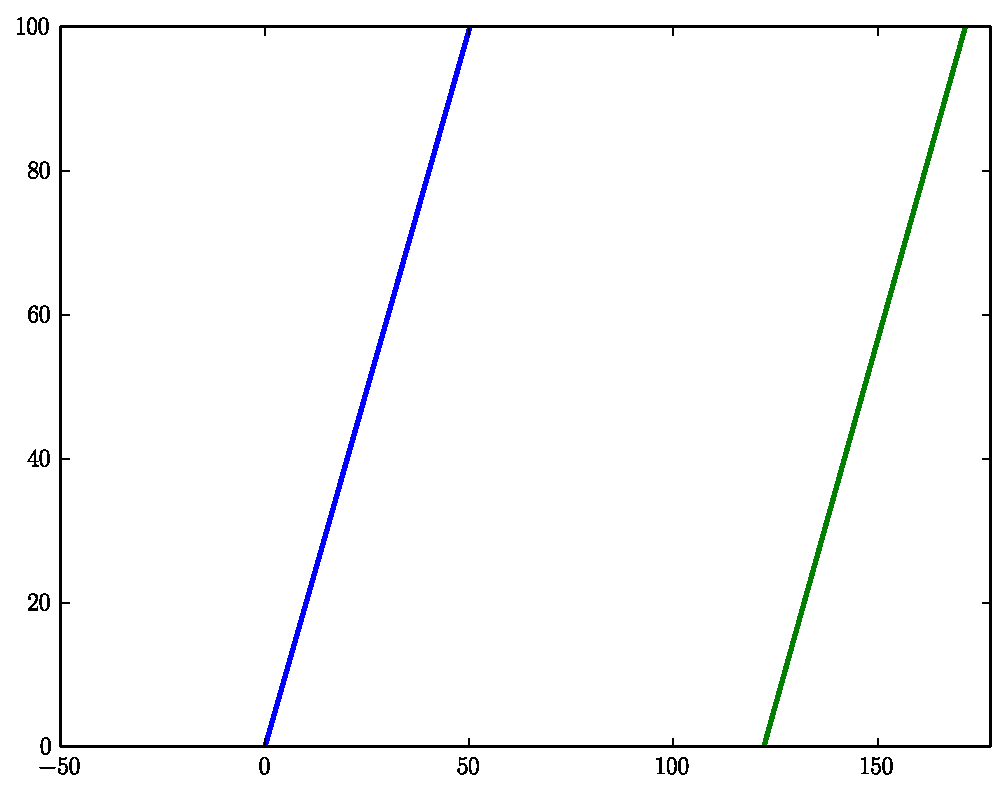
\includegraphics[width=.45\textwidth]{origin_micro}
    \end{tabular}
    \caption{Predicted vs. actual point of origin (detailed view on right).}
    \label{fig:origin}
\end{figure}

\begin{problem}
Add a function to you class that rewinds the system from a given state estimate, returning predictions for the previous states.
Do so by implementing the following function:
\begin{lstlisting}
def rewind(self,x,k):
    """
    Predict the k states preceding the current state estimate x.

    Parameters
    ----------
    x : ndarray of shape (n,)
        The current state estimate.
    k : integer
        The number of preceding states to predict.

    Returns
    -------
    out : ndarray of shape (n,k)
        The k preceding predicted states.
    """
    pass
\end{lstlisting}
\end{problem}

Returning to the projectile example, we can now predict the point of origin.

\begin{problem}
Using your state estimate $\widehat{\mathbf{x}}_{250}$, predict the point of origin of the projectile along with
all states leading up to time step $250$.
(The point of origin is the first point along the trajectory where the $y$ coordinate is $0$.)
Plot these predicted states (in cyan) together with the original state sequence.
Zoom in to see how accurate your prediction is.
Your plots should be similar to Figure \ref{fig:origin}.
\label{prob:origin_pt}

Repeat the prediction starting with $\widehat{\mathbf{x}}_{600}$.  Compare to the previous results.  Which is better?  Why?
\end{problem}
